%%%%%%%%%%%%%%%%%%%%%%%%%%%%%%%%%%%%%%%%%%%%%%%%%%%%%%%%%%%%%%%%%%%%%%%%%%%%%%
%%Skeleton LaTeX file: double column format.
%%%%%%%%%%%%%%%%%%%%%%%%%%%%%%%%%%%%%%%%%%%%%%%%%%%%%%%%%%%%
%%REMEMBER THAT THERES IS AN EIGHT PAGE SIZE RESTRICTION
%%%%%%%%%%%%%%%%%%%%%%%%%%%%%%%%%%%%%%%%%%%%%%%%%%%%%%%%%%%%

%%% Sample file for ME Project Papers for Evaluation by Supervisor and Reader

\documentclass{article}

\usepackage{multicol}
\usepackage{graphicx}

\pagestyle{empty}
\setlength{\topmargin}{ 0.25in}
\setlength{\columnsep}{2.0pc}
\setlength{\headheight}{0.0in}
\setlength{\headsep}{0.0in}
\setlength{\oddsidemargin}{-.19in}
\setlength{\parindent}{1pc}
\textheight 8.75in
\textwidth 6.8in

\title{\large \bf Predicting Query Execution Time }
\author{Name}

\date{}

\begin{document}

	\maketitle
    \begin{center}
        Mid-term ME Project Report
    \end{center}
        \vskip 12pt
	\thispagestyle{empty}
	
	\begin{abstract}
	The ability to estimate the query execution time is central for a number of tasks in database system
	such as query scheduling, progress monitoring and costing during query optimization. Recent work 
	has explored the use of statistical techniques in place of the manually constructed cost models used 
	in query optimization. Such techniques, which require as training data along with the 
	actual execution time, promises superior accuracies for they being able to account the for factors 
	such as hardware characteristics and bias in cardinality estimates. However, such techniques fail 
	to generalize i.e., produce poor estimates for queries that are not seen during the training.
	
	In this work, we propose and evaluate predictive modeling techniques that learn query 
	execution behavior at a fine grained operator level. For each operator, we consider different sets 
	of features and build different models for them. Since there are only finitely many operators in 
	database, this approach is practical and will be able to estimate any query as its a composition of
	many operators. We evaluate our approaches using TPC-H and TPC-DS workloads on PostgreSQL.

	\end{abstract}		
	\hfill 
	\begin{multicols}{2}
	\section{INTRODUCTION}
	Database systems can greatly benefit from accurate execution time predictions including: 
	\begin{itemize}
%	\item Query Optimizer: With accurate estimates, optimizer can rely on this metric to select the best plan among the many available plans.
	\item Admission control: Resource managers can use this metric to perform workload allocations such that the specific QoS are met \cite{activeSLA}.
	\item Query Scheduling: Knowing the execution time is crucial in deadline and latency aware 			scheduling
	\item Progress monitoring: Knowing the execution time of an incoming query can help avoid \textit{rogue queries} that are submitted in error and take an unreasonably long time to execute \cite{progress}.
	\end{itemize}
	Currently, execution time estimation is based on manually constructed
	models, which are part of the query optimizer and typically use
	combinations of weighted estimates of the number of tuples flowing
	through operators, column widths, etc. Unfortunately, such
	models often fail to capture several factors that affect the actual
	resource consumption. For example, they may not include detailed
	modeling of all of the various improvements made to database query
	processing – such as nested loop optimizations \cite{ganapathi, adaptive} which localize
	references in the inner subtree, and introduce “partially blocking”
	batch sorts on the outer side, thereby increasing the memory
	requirements and CPU time and reducing I/O compared to the traditional
	iterator model. Similarly, they may not accurately reflect
	specific hardware characteristics of the current production system
	or the impact of cardinality estimation errors. Analytical cost models predominantly 
	used by the current generation of query optimizers cannot
	capture these interactions and complexity; in fact, they are not designed to do so. 
	While they do a good job of comparing the costs of alternative query plans,
	they are poor predictors of plan execution latency. 
	Recent work \cite{ganapathi} showed this result for TPC-DS \cite{TPCDS}, and 
	in this work we do the same for TPC-H \cite{TPCH} data and queries.
	
	In this work, we utilize learning based models and prediction techniques which are promising reasonable accuracies in recent work \cite{ganapathi,MSR,ICDE2012}
	
	\section{Background:Model Based Prediction}	
COMEBACK:	Write about predictive stuff .. to give more intro. lets skip to imp parts now.

\hfill\\

	We use the term model to refer to any predictive function such as
	Multiple Regression, Bayesian Nets, and Support Vector Machines.
	Training a model involves using historical data sets to determine the
	best model instance that explains the available data. For example,
	fitting a function to a time series may yield a specific polynomial
	instance that can be used to predict future values.
	Model training (or building) requires selecting (i) the feature at-
	tributes, a subset of all attributes in the data set, and (ii) a predic-
	tion model, e.g., Linear Regression and Support Vector Machines
	(SVMs), to be used for modeling. In general, we cannot know
	which model type and feature set will produce the most accurate
	model for a given data set without building and testing multiple
	models. In some cases, a domain expert can manually specify the
	feature attributes. In other cases, this step is trivial as the prediction
	attribute(s) directly determine the feature attribute(s), e.g., in auto-
	regressive models. Alternatively, feature attributes can be learned
	automatically; however, given a set of n attributes, trying the power
	set is prohibitively expensive if n is not small or training is expen-
	sive [4, 3, 2] thereby requiring heuristic solutions.
	Most approaches rank the candidate attributes (often based on their
	correlation to the prediction attribute using metrics such as infor-
	mation gain or correlation coefficients) and use this ranking to guide
	
	a heuristic search [4] to identify most predictive attributes tested
	over a disjoint test data set. In this paper, we will use a similar For-
	ward Feature Selection algorithm based on linear correlation coef-
	ficients [4]. This algorithm essentially performs a best-first search
	in the model space. It starts with building models using small num-
	ber of features and iteratively builds more complex and accurate
	models by using more features. The features are considered with
	respect to their correlation with the target/prediction attribute. The
	training data set may be sampled to speed up the process.
	While we use a feature selection algorithm for building accurate
	models using relevant features, we do not consider building multi-
	ple models of different types for solving the model selection prob-
	lem. Instead in each one of our experiments we use a single type of
	prediction model, either Linear Regression or SVMs, that performs
	well.
	Hypothesis testing and confidence interval estimations are two com-
	mon techniques for determining predictive accuracy [2]. As men-
	tioned, it is not possible to estimate a priori what model would be
	most predictive for a given data set without training/testing it. One
	form of hypothesis testing that is commonly used is K-Fold Cross
	Validation (K-CV). K-CV divides the observed data up into k non-
	overlapping partitions. One of the partitions is used as validation
	data while the other k − 1 partitions are used to train the model
	and to predict the data in the validation interval. In this study, we
	will use cross-validation techniques to estimate the accuracy of our
	prediction models.

	\section{Overview of Proposed Approach}
	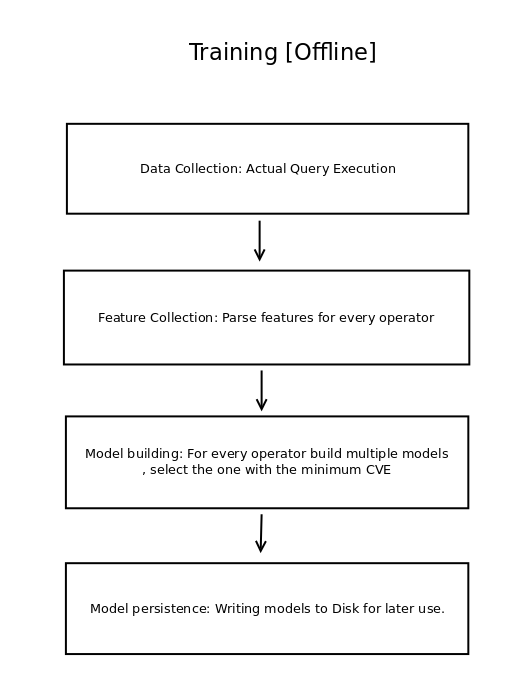
\includegraphics[scale=0.3]{training.png}
TODO :  
1. One more flowchart for Testing. 
2. Describe the concept of multiple models for a single operator. [MSR]
3. How do we select the best one among them. (Mention that current experiments dont use this idea, only one a simple non-linear model is used for all models with 2 features) 


	Elaborate what is the plan level approach. give  a intro model
	 based techniques. i.e.,  OFF LINE TRAINING, emphasize one time.
	1. How to obtain training data (explain analyze)
	2. getting execution times at plan nodes
	3. Individual model training 
	4. Explain while testing and predict using Model more in next section
	
	
	
	Mention assumptions, 
	Pure in-memory.. lets solve this first.
	For example, a sort merge


join may require sorting its inputs. The sort operators are then responsible for
handing over their result to the merge join via main memory. This means that
the merge join may not require any I/O if the merge can be done purely in
main memory

Analytical approaches problems: 

counting the numbers of pages read is not
sufficient as the discrepancy between random and sequential I/O is tremendous.

%%%%%%%%%%%%%  This can be followed by several other sections
	\section{Model selection and Training}
	What model is considered good ? choice of model and kernel
	If possible prove linear systems are not sufficient.
	Training data ,specification. Does more training data helps?
	 training time etc.. 
	Essentially all operators need to be covered. generation QGEN tool. 
	\section{Preliminary Experiments}
	
	If possible plot a non-linear SVR for the data. will the optimizer's cost 
	itself is enough 1D regression using linear, polynomial and RBF kernels
	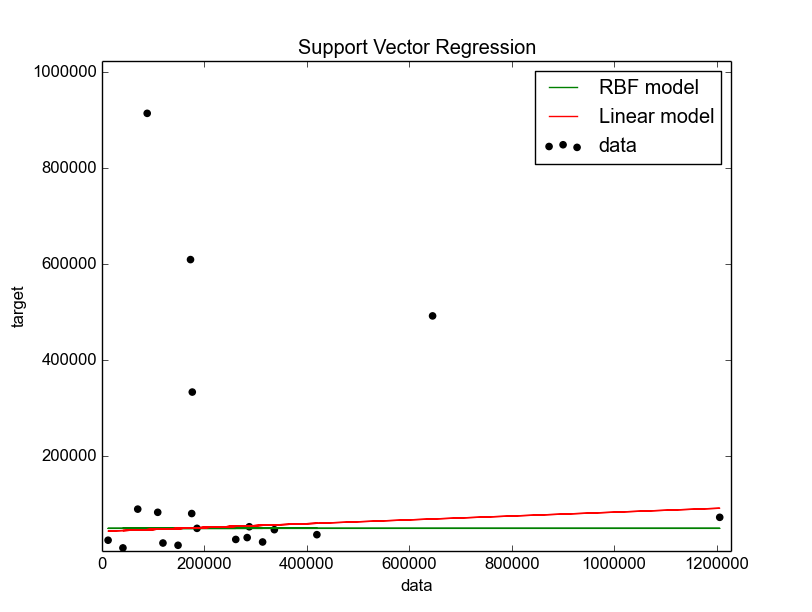
\includegraphics[scale=.33]{optcost.png}  
	
	
	Give a background about Static and dynamic workload.  
	do experiments at 2 stages
	1. Act vs Act
	2. Est vs Est(Bias towards estimated cardinalities)
	For each type of above scenario, do testing for tpc-h queries 
	(tpc-ds in future)
	At different scales to see the model's ability to predict.
	For midterm you should be having result for 1 as well as 10 GB.
	For each above dataset, 
	Results should convey L1 (MRE) as well as queries that are within 
	[0-0.5] [0.5-1] [1-1.5] 
	\section{Conclusions and Future Work}
	Talk about generalization. 
	operator specific features
	capturing query interaction i.e., pipeline source of over-estimation
	Optimizers provides sufficient information to detect a pipeline,
	 can we use it to bind the operators and predict execution time 
	 for a set of operators instead of a single operator.
	
	\begin{thebibliography}{9}
	\bibitem{opthet} 
	Du, Weimin, Ravi Krishnamurthy, and Ming-Chien Shan. "Query optimization in a heterogeneous dbms." 		VLDB. Vol. 92. 1992.
	\bibitem{activeSLA}
	Xiong, Pengcheng, et al. "ActiveSLA: a profit-oriented admission control framework for database-as-a-		service providers." Proceedings of the 2nd ACM Symposium on Cloud Computing. ACM, 2011.	
	\bibitem{progress}
	Mishra, Chaitanya, and Nick Koudas. "The design of a query monitoring system." ACM Transactions on 		Database Systems (TODS) 34.1 (2009): 1.
	
	\bibitem{ganapathi} 
	A. Ganapathi, H. A. Kuno, U. Dayal, J. L. Wiener, A. Fox, M. I. Jordan,
	and D. A. Patterson. Predicting multiple metrics for queries: Better
	decisions enabled by machine learning. In ICDE, 2009.
	
	\bibitem{MSR}
	Li, Jiexing, et al. "Robust estimation of resource consumption for sql queries using statistical 			techniques." Proceedings of the VLDB Endowment 5.11 (2012): 1555-1566.
	
	\bibitem{ICDE2012}
	Akdere, Mert, et al. "Learning-based query performance modeling and prediction." Data Engineering 			(ICDE), 2012 IEEE 28th International Conference on. IEEE, 2012.	
	
     \bibitem{adaptive} 
     S. Guirguis, M. A. Sharaf, P. K. Chrysanthis, A. Labrinidis, and
	K. Pruhs. Adaptive scheduling of web transactions. In ICDE, 2009.

	\bibitem{TPCH}
	TPC-H benchmark specification, http://www.tpc.org/tpch/
	
	\bibitem{TPCDS}
	R. Othayoth and M. Poess, The making of tpc-ds, in VLDB
	06: Proceedings of the 32nd international conference on Very
	large data bases. VLDB Endowment, 2006, pp. 1049Ð1058

	\end{thebibliography}
	\end{multicols}
\end{document}
